\section{Overview} %%%%%%%%%%%%%%%%%%%%%%%%%%%%%%%%%%%%%%%%%%%%%%%%%%
\label{sec:over}

A \emph{hierarchy} is a partially ordered set $(H,\subtype)$ where $H$ is a set 
of classes and $\subtype$ is reflexive, transitive and anti-symmetric 
\emph{subtyping relation}. We are going to use terms \emph{class} and \emph{type} 
interchangibly as the exact distinction is not important for this discussion. 
Given two types in a subtyping relation $D \subtype B$, type $D$ is said to be a 
\emph{subtype} or \emph{derived class} of $B$, which in turn is said to be a 
\emph{supertype} or \emph{base class} of $D$.

Subtyping effectively makes objects belong to multiple types. We call by the 
\emph{most-derived type} the type used to create an object (before any 
conversions). By \emph{static type} we call the type of an object as known to 
the compiler based on its declaration as well as any supertype of it. By 
\emph{dynamic type} of an object we call any base class of the most-derived type.

\subsection{Type Switch}

%This section generalizes pattern matching of closed algebraic datatype values
%to case analysis of hierarchical and extensible datatype values.
In general, \emph{type switch} or \emph{typecase} is a multiway branch statement 
that distinguishes values based on their type. In a multi-paradigm programming 
language like C++ that supports in various forms parametric, ad-hoc and 
subtyping polymorphisms, such a broad definition subsumes numerous different type 
casing constructs studied in the literature~\cite{Intensional95,Glew99,OpenShutTypecase05}. 
In this work we only look at type casing scenarios based on dynamic polymorphism 
of C++ (nominative subtyping polymorphism based on inheritance), similar to 
those studied by Glew~\cite{Glew99}. It is possible to generalize type casing 
(the notion, not our implementation) to static polymorphism of C++ (ad-hoc and 
parametric polymorphisms enabled by overloading and templates) along the line of 
work introduced by Harper and Morrisett~\cite{Intensional95} and studied in the
context of closed and extensible solutions by Vytiniotis et 
al~\cite{OpenShutTypecase05}, but we do not address such a generalization here. 
We use the term \emph{type switch} instead of a broader \emph{typecase} to 
stress the run-time nature of the type analysis similar to how regular 
\code{switch}-statement of C++ performs case analysis of values at run time.

Given an object descriptor, called \emph{subject}, of static type \code{S} 
(pointer or reference) referred to as \emph{subject type}, and a list of 
\emph{target types} \code{Ti} associated with the branches, a type switch 
statement needs to identify a suitable clause $m$ (or absence of such) based on 
the most-derived type \code{D <: S} of the subject as well as properly adjusted 
reference to the target type \code{Tm}. 
Due to multiple inheritance, types \code{Ti} in general may or may not be 
derived from \code{S}, however, because of the strong static type safety 
requirement, the type of applicable clause \code{Tm} will necessarily have to be 
one of subject's dynamic types: \code{D <: Tm}. A hypothetical type switch 
statement, not currently supported by C++, may look as following:

\begin{lstlisting}[keepspaces]
switch (subject) { case T1: s1; ... case Tn: sn; }
\end{lstlisting}

\noindent
There is no need for an explicit \emph{default clause} in our setting because 
such a clause is semantically equivalent to a case clause guarded by the 
subject type: \code{case S: s}. The only semantic difference such a choice 
makes is in the treatment of null-pointers, which, one may argue, should be 
handled by the default clause. We disagree, because not distinguishing between 
invalid object and valid object of a known static but unknown dynamic type may 
lead to some nasty run-time errors.

Similar control structures exist in many programming languages, e.g. 
\emph{match} in Scala~\cite{Scala2nd}, \emph{case} in Haskell~\cite{} and 
ML~\cite{}, \emph{typecase} in Modula-3~\cite{Modula3TS} and CLOS~\cite{} (as a 
macro), \emph{tagcase} in CLU~\cite{CLURefMan}, \emph{union case} in Algol 68 
and date back to at least Simula's \emph{Inspect} statement~\cite{Simula67}. 
The statement in general can be given numerous plausible semantics:

\begin{itemize}
\setlength{\itemsep}{0pt}
\setlength{\parskip}{0pt}
\item \emph{First-fit} semantics will evaluate the first statement $s_i$ such 
      that $T_i$ is a base class of $D$
\item \emph{Best-fit} semantics will evaluate the statement corresponding to the 
      most-derived base class $T_i$ of $D$ if it is unique (subject to 
      ambiguity)
\item \emph{Exact-fit} semantics will evaluate statement $s_i$ if $T_i=D$.
\item \emph{All-fit} semantics will evaluate all statements $s_i$ whose guard 
      type $T_i$ is a subtype of $D$ (order of execution has to be defined)
\item \emph{Any-fit} semantics might choose non-deterministically one of the 
      statements enabled by all-fit
\end{itemize}

\noindent
The list is not exhaustive and depending on a language, any of these semantics 
can be a plausible choice. Functional languages, for example, often prefer 
first-fit semantics because it is similar to case analysis in mathematics. 
Object-oriented languages would typically be inclined to best-fit semantics due 
to its similarity to overload resolution and virtual dispatch, however, some 
do opt for first-fit semantics to mimic the functional style: e.g. Scala~\cite{Scala2nd}. 
Exact-fit semantics can often be seen in languages supporting discriminated 
union types: e.g. variant records in Pascal, Ada and Modula-2, oneof and variant 
objects in CLU, unions in C and C++ etc.
All-fit and any-fit semantics might be seen in languages based on predicate 
dispatching~\cite{ErnstKC98} or guarded commands~\cite{EWD:EWD472}, where a 
predicate can be seen as a characteristic function of a type, while logical 
implication can be seen as subtyping.

\subsection{Expression Problem}

Type switching is related to a more general problem manifesting the differences 
in functional and object-oriented programming styles.

%The ideas and the library were motivated by our unsatisfactory experiences 
%working with various C++ front-ends and program analysis 
%frameworks~\cite{Pivot09,Phoenix,Clang}.
%The problem was not in the frameworks per se, but in the fact that we had to use
%the \emph{visitor design pattern}~\cite{DesignPatterns1993} to inspect, traverse, and 
%elaborate abstract syntax trees to target languages. We found visitors 
%unsuitable to express our application logic directly, surprisingly hard to teach 
%students, and often slower than hand-crafted workaround techniques. Use of 
%dynamic casts in many places, often nested, to answer simple structural 
%questions, shows that the users preferred shorter, cleaner, and more direct code 
%to visitors, even at a high cost in performance (providing they understood the cost).
%
%A lot has been written about the visitor design pattern~\cite{DesignPatterns1993,Palsberg98,Zenger:2001,Oliveira08}. 
%Its advantages include \emph{extensibility of functions}, \emph{speed}, and, 
%\emph{being a library solution}. Nevertheless, the solution is \emph{intrusive}, 
%\emph{specific to hierarchy}, and requires a lot of \emph{boilerplate code} to 
%be written. It also introduces \emph{control inversion}, and, most importantly, 
%-- \emph{hinders extensibility} of classes.
%Interestingly, as bad as visitors are, they are only trying to solve a larger 
%problem in the context of object-oriented languages.

%Expression problem is a problem of supporting in a programming language modular 
%extensibility of both data and functions at the same time. Functional languages
%allow for easy addition of new functions at the expense of disallowing new data
%variants. Object-oriented languages allow for easy addition of new variants at 
%the expense of disallowing new functions. Many attempts have been made to 
%resolve this dilema in both camps, nevertheless no universally accepted solution 
%that is modular, open and efficient has been found.

%Visitor Design Pattern has became de-facto standard in dealing with expression 
%problem in many industry-strength object-oriented languages because of two 
%factors: its speed and being a library solution. It comes at the cost of 
%restricting extensibility of data, increased verbosity and being hard to teach 
%and understand, but nevertheless, remains the weapon of choice for interacting 
%with numerous object-oriented libraries and frameworks. 

Conventional algebraic datatypes, as found in most functional languages, allow 
for easy addition of new functions on existing data types. But they fall short 
in extending data types themselves (e.g. with new constructors), which requires 
modifying the source code. Object-oriented languages, on the other hand, make 
data type extension trivial through inheritance; but the addition of new 
functions operating on these classes typically requires changes to the class 
definition. This dilemma is known as the \emph{expression problem}~\cite{Cook90,exprproblem}.

Classes differ from algebraic data types in two important ways. Firstly, they
are \emph{extensible}, for new variants can be added later by inheriting from
the base class. Secondly, they are \emph{hierarchical} and thus typically 
\emph{non-disjoint} since variants can be inherited from other variants and form 
a subtyping relation between themselves~\cite{Glew99}. In contrast, variants in 
algebraic data types are \emph{disjoint} and \emph{closed}.
Some functional languages e.g. ML2000~\cite{ML2000} and its predecessor, Moby, 
were experimenting with \emph{hierarchical extensible sum types}, which are 
closer to object-oriented classes then algebraic data types are, but, 
interestingly, they provided neither traditional nor efficient facilities for 
performing case analysis on them.

Zenger and Odersky later refined the expression problem in the context of 
independently extensible solutions~\cite{fool12} as a challenge to find an 
implementation technique that satisfies the following requirements:

\begin{itemize}
\setlength{\itemsep}{0pt}
\setlength{\parskip}{0pt}
\item \emph{Extensibility in both dimensions}: It should be possible to add new 
      data variants, while adapting the existing operations accordingly. It 
      should also be possible to introduce new functions. 
\item \emph{Strong static type safety}: It should be impossible to apply a 
      function to a data variant, which it cannot handle. 
\item \emph{No modification or duplication}: Existing code should neither be 
      modified nor duplicated.
\item \emph{Separate compilation}: Neither datatype extensions nor addition of 
      new functions should require re-typechecking the original datatype or 
      existing functions. No safety checks should be deferred until link or 
      runtime.
\item \emph{Independent extensibility}: It should be possible to combine 
      independently developed extensions so that they can be used jointly.
\end{itemize}

\noindent
While these requirements were formulated for extensible data type with 
disjoint variants, object-oriented languages primarily deal with 
hierarchical data types. We thus found it important to explicitly state an 
additional requirement based on the Liskov substitution principle~\cite{Lis87}:

\begin{itemize}
\setlength{\itemsep}{0pt}
\setlength{\parskip}{0pt}
\item \emph{Substitutability}: Operations expressed on more general data variants
      should be applicable to more specific ones that are in a subtyping relation 
      with them.
\end{itemize}

%Depending on the semantics of the language's subtyping relation, 
%substitutability requirement may turn pattern matching into an expensive 
%operation. OCaml, for example, that uses structural subtyping on its object 
%types, does not offer pattern 

\noindent
We will refer to a solution that satisfies all of the above requirements as \emph{open}. 
Numerous solutions have been proposed to dealing with the expression problem in both 
functional~\cite{garrigue-98,LohHinze2006} and object-oriented 
camps~\cite{Palsberg98,Krishnamurthi98,Zenger:2001,runabout}, but very few has 
made its way into one of the mainstream languages. We refer the reader to Zenger 
and Odersky's original manuscript for a discussion of the approaches~\cite{fool12}.
Interestingly, most of the discussed object-oriented  
solutions were focusing on the visitor design pattern and its extensions, 
which even today seems to be the most commonly used approach to dealing with the 
expression problem in object-oriented languages.

A lot has been written about the visitor design pattern~\cite{DesignPatterns1993,Palsberg98,Zenger:2001,Oliveira08}. 
Its advantages include \emph{extensibility of functions}, \emph{speed}, and, 
\emph{being a library solution}. Nevertheless, the solution is \emph{intrusive}, 
\emph{specific to hierarchy}, and requires a lot of \emph{boilerplate code} to 
be written. It also introduces \emph{control inversion}, and, most importantly, 
-- \emph{hinders extensibility} of classes.

%In this work we are not trying to solve the expression problem in its full 
%generality. Instead, we concentrate on deficiencies of the visitor design 
%pattern independently of its relation to the expression problem and advocate for 
%a solution that suits object-oriented paradigm better than visitors do.

\subsection{Open Type Switch}

Note that the presence of a type switch in an object-oriented language alone 
does not solve the expression problem because the existing code may have to be 
modified to take new variants into account. Relying on default clause is not 
considered to be an acceptable solution in this context, because often times the 
only reasonable default behavior is to raise an exception. Zenger and Odersky 
note that in such cases defaults will transform type errors that should manifest 
statically into runtime exceptions that are thrown dynamically~\cite{fool12}.

While we generally agree with this observation, we would like to point out that 
in our experience newly added variants were more often extending an existing 
variant than creating an entirely disjoint one. In a hypotetical compiler, for 
example, a new kind of type expression will typically extend a 
\code{TypeExpression} variant, while a new form of annotation will extend an 
\code{Annotation} variant, thus not extending the root \code{ASTNode} directly. 
Due to substitutability requirement such a new variant will be treated as a 
variant it extends in all the existing code. The functions that will be affected 
by its addition and thus have to be modified will be limited to functions 
directly analyzing the variant it extends and not providing a default behavior.

To account for this subtlety of extensible hierarchical data types, we use a 
term \emph{open type switch} to refer to a type switch that satisfies all the 
requirements of an \emph{open solution to expression problem} stated above 
except for the \emph{no modification or duplication} requirement. We loosen it 
to allow modification of functions for which the newly added variant becomes a 
disjoint (orthogonal) case not handled by default clause. We believe that the 
loosened requirement allows us to express pragmatically interesting restrictions 
that developers are willing to live with. Besides, open type switch overcomes 
all the major shortcomings of the visitor design pattern:

\begin{itemize}
\setlength{\itemsep}{0pt}
\setlength{\parskip}{0pt}
\item Case analysis with an open type switch is \emph{non-intrusive} as it 
      inspects the hierarchy externally and can be applied retroactively. 
\item New variants can be accounted for in the newly written code and will be 
      seen as a base class or default in the existing code.
\item The affected functions are limited to those for which the newly added 
      variant is a disjoint case.
\item The code avoids the control inversion and the need for boilerplate code 
      that visitors introduce, and is thus a more direct expression of the 
      intent.
\end{itemize}

\section{Problem Description} %%%%%%%%%%%%%%%%%%%%%%%%%%%%%%%%%%%%%%%%%%%%%%%%%%
\label{sec:probl}

\subsection{Previous Work}
\label{sec:prev}

The closed nature of algebraic data types allows for their efficient 
implementation. The traditional compilation scheme assigns unique (and often 
small and sequential) tags to every variant of the algebraic data type and type 
switching is then simply implemented with a multi-way branch~\cite{Spuler94} 
(usually a jump table) over all the tags~\cite{Augustsson85}. Dealing with 
extensible hierarchical data types makes this extremely efficient approach 
infeasible:

\begin{itemize}
\setlength{\itemsep}{0pt}
\setlength{\parskip}{0pt}
\item \emph{Extensibility} implies that the compiler may not know the exact set 
      of all the derived classes till link-time (due to \emph{separate compilation}) 
      or even run-time (due to \emph{dynamic linking}).
\item \emph{Substitutability} implies that we should be able to 
      match tags of derived classes against case labels representing tags of 
      base classes.
\item Presence of \emph{multiple inheritance} might require pointer adjustments 
      that are not known at compile time (e.g. due to virtual base classes, 
      ambiguous base classes or cross-casting).
\end{itemize}

%\noindent
%In some cases the substitutability requirement can be satisfied by obtaining 
%the base class' tag from a derived one first and then performing the jump. 
%This will work as long as we have only base classes in the case clauses.
%Derived classes that have to be treated separately from the rest of their 
%siblings will essentially be indistinguishable from them.
%
%When tags are not chosen arbitrarily but to reflect the subtyping relation of the 
%underlying hierarchy (e.g. certain bit set for certain base class), the assumed 
%structure of tags is likely to make the set of tags sparse. On one hand this 
%decreases the number of representable hierarchies and thus hinders openness, 
%while on the other it forces the compiler to use a decision tree instead of a jump 
%table to implement the switch. The former was consistently slower than the 
%latter one in our experience, even though the opposite was noted on some 
%architectures for small number of case clauses~\cite[\textsection 4]{garrigue-98}.

\noindent
There are two main approaches to implementing case analysis on extensible 
hierarchical data types, discussed in the literature.

The first approach is based on either explicit or implicit sealing of the class 
hierarchy, on which type switching can be performed. In Scala, for example, the 
user can forbid future extensions from a given class hierarchy through the use 
of a \code{sealed} keyword~\cite[\textsection 4.3.2]{EmirThesis}. The compiler 
then uses the above tag allocation over all variants to implement type analysis.
In some cases the sealing may happen implicitly. For example, languages that 
allow names with internal and external linkage may employ the fact that classes 
with internal linkage will not be externally accessible and thus effectively 
sealed. While clearly efficient, the approach is not open as it avoids the 
question rather than solves. 

The broader problem with this approach is that techniques that rely on unique or
sequential compile or link-time constants violate independent extensibility 
since without a centralized authority there is no guarantee same constant will 
not be chosen in type unsafe manner by independent extensions. Updating such 
constants at load time may be too costly even when possible. More often than 
not however such updates may require code regeneration since decision trees, 
lookup tables etc. may have been generated by compiler for given values.

An important practical solution that follows this approach is the visitor design 
pattern~\cite{DesignPatterns1993}. The set of \code{visit} methods in visitor's 
interface essentially seals the class hierarchy. Extensions have been proposed 
in the literature~\cite{Zenger:2001}, however they have problems of their own, 
discussed in \textsection\ref{sec:rw}.

The second approach employs type inclusion tests combined with decision 
trees~\cite{Cardelli84} to avoid duplicate checks. The efficiency of the 
approach is then entirely focused on the efficiency of type inclusion 
tests~\cite{Schubert83,Wirth88,Cohen91,Caseau93,Vortex96,Krall97nearoptimal,Vitek97,PQEncoding,FastDynCast,Ducournau08}.

Type inclusion tests for single inheritance were initially implemented by 
traversing a linked list of types, as proposed by Wirth~\cite{Wirth88}. Such 
encoding requires little space, but runs in time proportional to the distance 
between the two types in the class hierarchy. A trivial constant-time type 
inclusion test can be achieved with a \emph{binary matrix}, encoding the 
subtyping relation on the class hierarchy~\cite{Vortex96}. While efficient in 
time, it has quadratic space requirements, which makes it expensive for use on 
large class hierarchies. In response to Wirth' original publication, Cohen 
proposed the first space-efficient constant-time algorithm, which, howver, could 
only deal with single inheritance~\cite{Cohen91}. \emph{Hierarchical encoding} 
is another constant-time test that maps subtype queries into subset queries on 
bit-vectors~\cite{Caseau93,Krall97nearoptimal}. The approach can handle multiple
inheritance, but the space and time required for a subtype test in this encoding 
increases with the size of the class hierarchy, also Caseau's approach is 
limited to class hierarchies that are lattices. Schubert's \emph{relative 
numbering}~\cite{Schubert83} encodes each type with an interval $[l,r]$, 
effectivelly making type inclusion tests isomorphic to a simple range checking. 
The encoding is optimal in space and time, however it is limited to single 
inheritance. \emph{PQ-Encoding} of Zibin and Gil employs PQ-trees to improve 
further space and time efficiency of the constant-time inclusion 
testing~\cite{PQEncoding}. While capable of handling type inclusion queries on 
heterarchies, the approach makes the closed world assumption and can be costly 
for use with dynamic linking because it is not incremental.
The approach of Gibbs and Stroustrup~\cite{FastDynCast} employs divisibility of 
numbers to obtain a constant-time type inclusion test. The approach can handle 
multiple inheritance and was the first constant-time technique to addresses the 
problem of the this-pointer offsets. Unfortunately the approach limits the size 
of the class hierarchies that can be encoded with this technique. 
Ducournau proposed constant-time inclusion test based on the fact that in an 
open solution a class has known amount of base classes and thus perfect hashes 
can be used to map them to this-pointer offsets\cite{Ducournau08}. Unfortunately 
the approach addresses only virtual multiple inheritance and similarly to other 
approaches relies on load-time computations that may be costly.
Detailed analysis and explanation of existing constant-time type inclusion tests 
can be found in \cite{Vitek97} and \cite{PQEncoding}.

With the exception of work by Gibbs and Stroustrup~\cite{FastDynCast}, all the 
approaches to efficient type-inclusion testing we found in the literature were 
based on the assumption that \emph{the outcome of a subtyping test as well as 
the subsequent cast depend only on the target type (type being queried) and the 
most-derived type of the object}. While such assumption is sound for describing 
a subtyping relationship between two types, it does not fully reflect the 
relationship between subobjects of the same object, induced by the inheritance 
relation of the language. % We elaborate in the next section.

\subsection{The Devil is in the Details: Casts}
\label{sec:casts}

%There is a tight coupling between subtype testing and type casting. When two 
%types are in subtyping relation, we expect to be able to cast between these two 
%types of the same object. When such cast is not possible due to semantic 
%reasons, our subtyping relation is not anymore in sync with casting.
%
%\begin{itemize}
%\setlength{\itemsep}{0pt}
%\setlength{\parskip}{0pt}
%\item Subtyping and inheritance are two distinct relationships (in C++ at least)
%\item Type casts and subtype tests are tightly coupled when subtyping differs 
%      from inheritance
%\end{itemize}

%Following the notion of Wasserrab et al~\cite{WNST06}, in a given program $P$, 
%a class $B$ is a \emph{direct repeated base class} of $D$ if $B$ is mentioned in 
%the list of base classes of $D$ without the \code{virtual} keyword ($D \prec_R B$).
%Similarly, a class $B$ is a \emph{direct shared base class} of $D$ if $B$ is mentioned in 
%the list of base classes of $D$ with the \code{virtual} keyword ($D \prec_S B$). 
%A reflexive transitive closure of these relationships $\preceq^*=(\prec_R \cup \prec_S)^*$ 
%defines the \emph{inheritance} relation on types of program $P$.

Interestingly enough, none of the constant-time type-inclusion techniques 
discussed in the literature are used by the industry C++ compilers, which
instead resort to variations of Wirth' original idea extended to multiple 
inheritance. To understand why, it is important to observe that type inclusion 
tests are rarely useful by themselves and are followed most of the time by a 
type cast to obtain a valid reference. To stress this coupling of type inclusion 
tests and type casts, C++ provides only a single operation \code{dynamic_cast} 
that combines them both~\cite[\textsection 14.2.2]{Str94}. This is not the case 
in many other object-oriented languages, e.g. Java, where type testing with 
\code{instanceof} is independent of type casting. When type testing is 
independent of type casting, there is usually an implicit premise that 
\emph{success of a type test implies the success of a corresponding cast}. When 
such a premise cannot be guaranteed due to some reasons, we are not anymore 
interested in testing whether two types are in a subtyping relation, but whether 
a conversion is possible. Implementation of such a test is likely to be similar 
to the implementation of the actual cast, in which case it makes sense to 
combine them. Support of repeated multiple inheritance in C++ gives rise to 
examples where the conversion between two types in subtyping relation is not 
possible and thus the above premise cannot be guaranteed.  

%Both approaches have their pros and cons. When 
%major parts of the subtype test are also parts of the cast's implementation, the 
%compiler may need to do some non-trivial static analysis in order to infer 
%whether the user has already estblished the subtyping relation for a given cast 
%and whether intermediate results can be reused in the cast's implementaiton. On 
%the other hand, such separation of concerns may be useful in code that expects a 
%lot of negative outcomes from subtype tests, thus letting each specific test 
%fail earlier. The C++ approach stresses that these two operations are highly 
%coupled both in use and their implementation and thus combines them into a 
%single operator.

%For single inheritance, the cast is usually a no-op once the inclusion has been 
%esteblished, but for multiple inheritance it often involves a non-constant 
%run-time overhead, in which case the complexity of the combined operation 
%should be studied instead. In some cases corresponding constant-time encoding 
%can be augmented with information necessary for the subsequent cast. In case of 
%binary matrix encoding, for exampple, we may keep the necessary offsets along 
%with the subtyping relation, however the space requirements will become even 
%less tolerable. With the exception of fast dynamic cast of Gibbs and Stroustrup 
%as well as perfect hashing of Ducournau, none of the work on constant-time 
%subtype testing capable of handling multiple inheritance addresses the 
%efficiency of type casting once the type inclusion has been established. It was 
%also not immediately obvious how the techniques can be adopted to account for 
%casting without significantly affecting the established time or space 
%complexity.

\begin{figure}[htbp]
  \centering
    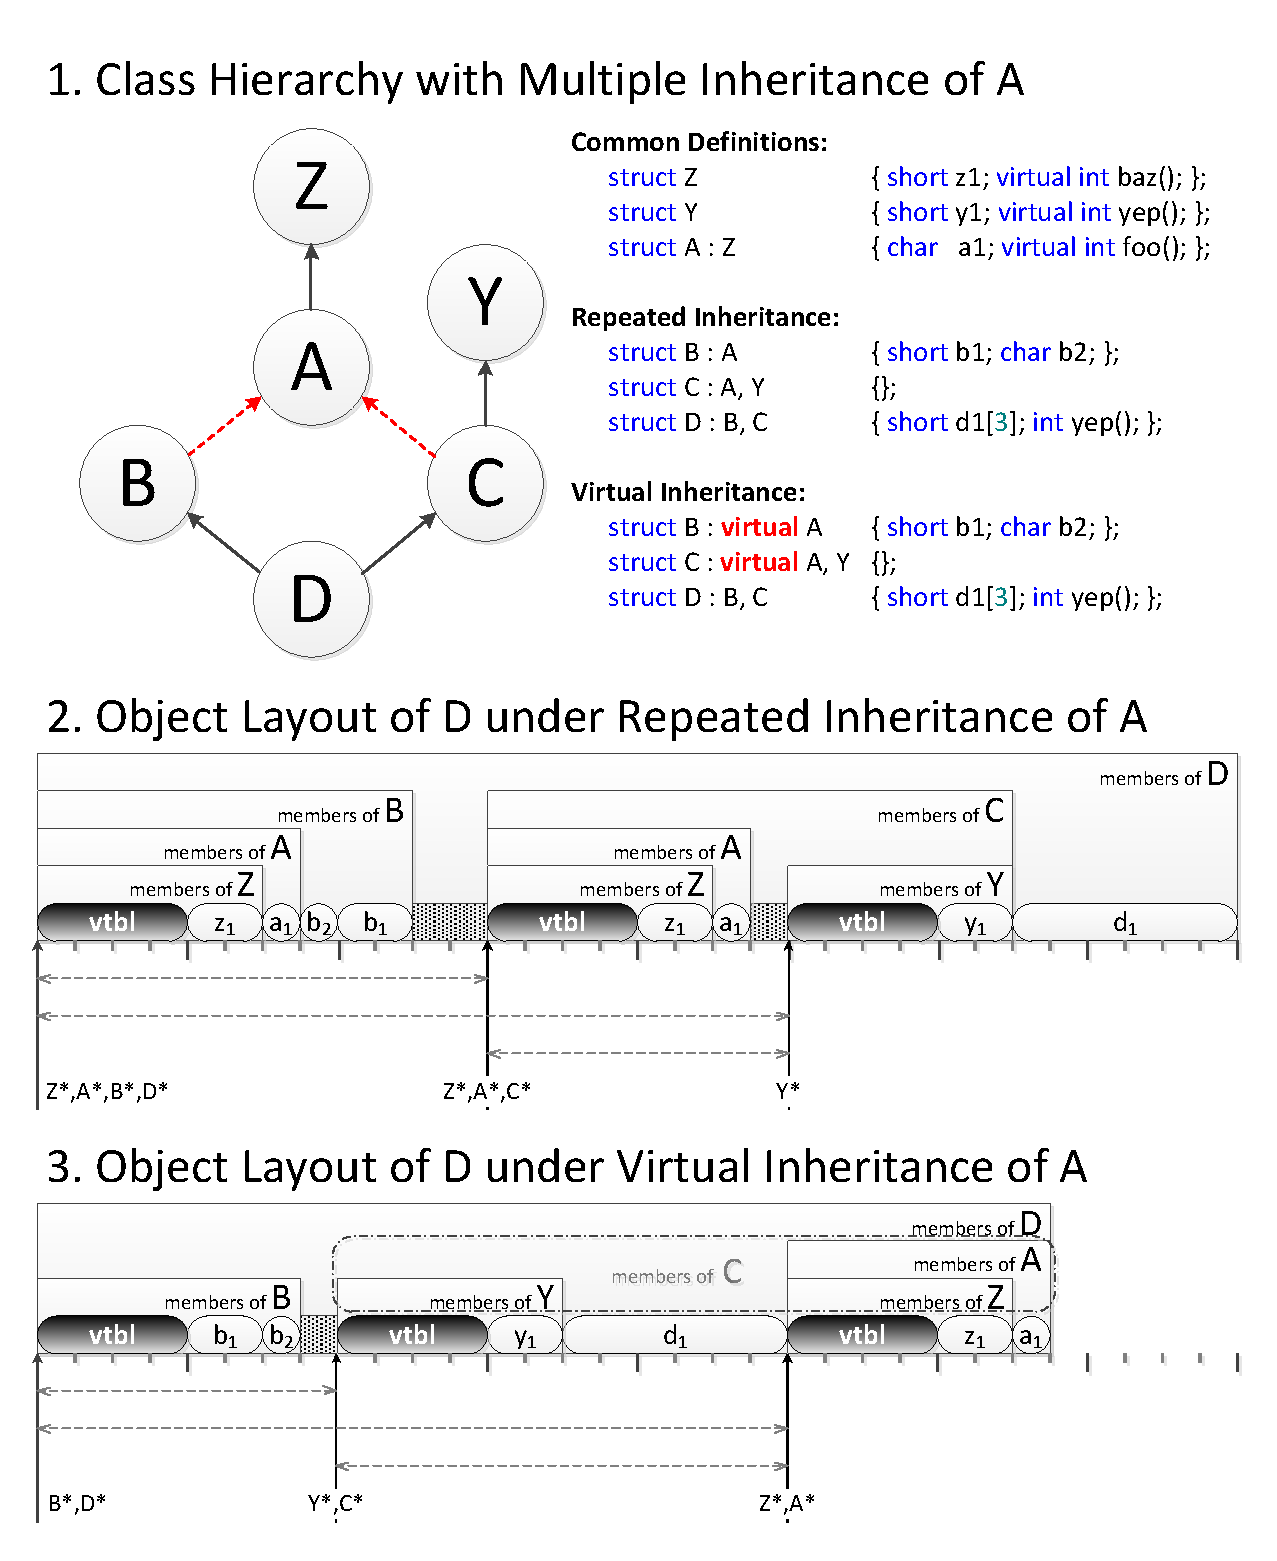
\includegraphics[width=0.47\textwidth]{Classes.pdf}
  \caption{Object Layout under Multiple Inheritance}
  \label{fig:objlayout}
\end{figure}

Consider a simple class hierarchy in Figure~\ref{fig:objlayout}(1). To better 
support multiple inheritance, classes in C++ may inherit from other classes 
directly or virtually. When certain base class is inherited via multiple 
inheritance pathes, as is the case with \code{D} inheriting \code{A} through its 
\code{B} and \code{C} base classes, the user may opt to keep distinct 
sub-objects of class \code{A} (repeated multiple inheritance) or a shared one 
(virtual multiple inheritance) by specifying how \code{B} and \code{C} are 
inherited from \code{A}. A typical object layout generated for class \code{D} in 
each of these cases is shown in parts (2) and (3) of the 
Figure~\ref{fig:objlayout} respectively.

Due to extensibility of classes, the layout decisions for classes have to be 
made independently of their derived classes. In turn, the layout of derived 
classes must conform to the layout of its base classes relatively to the offset 
of the base class within derived. For example, the layout of \code{A} within 
\code{C} is exactly the same as the layout of \code{A} in \code{B} and is simply 
the layout of \code{A}. Base classes inherited virtually do not contribute to 
the fixed layout because they are looked up indirectly at run-time to ensure 
that only one shared instance of such a base class exists in the derived class. 
Because of this indirection, virtual inheritance incures slight overhead at 
run-time.

Under single (non-virtual) inheritance members of the base class are typically 
layed out before the members of derived class resulting in the base class being 
at the same offset as the derived class itself. In our example, the offset 
of \code{A} in \code{B} under regular (non-virtual) inheritance of \code{A} is 0.  

Under multiple inheritance, different base classes might be at different offsets 
in the most-derived class, which is why pointers of a given static type may only 
be pointing to certain positions in it. These positions are marked in the 
picture with vertical arrows decorated with the set of pointer types whose 
values may point into that position. Run-time conversions between such pointers 
represent conversions between different dynamic types of the same most-derived 
type and may require adjustments to this-pointer (shown with horizontal dashed 
arrows) to maintain type safety. Such conversions can be generally categorized 
into 3 categories: upcasts, downcasts and crosscasts.

An \emph{upcast} is a cast from a derived class to one of its bases. When the 
base class is unambiguous, such casts are implicit and require no additional 
annotations. When the base class is ambiguous, as is the case when casting 
\code{D} to \code{A} under repeated multiple inheritance of \code{A}, the user 
needs to explicitly cast the object to \code{B} or \code{C} first in order to 
indicate the desired subobject. Upcasts to non-virtual base class usually 
require no additional instructions or an instruction performing adjustment of 
this-pointer by a statically known constant. Upcasts to virtual base class 
require an adjustment to this-pointer by a value looked up dynamically.

A \emph{downcast} is a cast from a base class to one of its derived classes. The 
cast requires run-time checking of whether object's most-derived type inherits 
from requested derived class. Downcasts in C++ have to be made explicit through 
the use of operator \code{T* dynamic_cast<T*>(S* s)}, which takes a querried 
dynamic type \code{T} and a pointer \code{s} to object of polymorphic type 
\code{S}. It returns \code{nullptr} when the requested type is not one of 
object's dynamic types, otherwise a properly adjusted pointer to dynamic type 
\code{T} of the object.

A \emph{crosscast} is a cast between classes not related by inheritance. Similar 
to downcast it is performed with the help of \code{dynamic_cast}, while its 
semantics is defined to be a composition of upcast to target type and downcast 
to the most-derived type \code{D}: i.e. \code{(T*)dynamic_cast<D*>(s)}. While 
the downcast is guaranteed to succeed in this case, the upcast may be ambiguous, 
in which case the result will be \code{nullptr}.

While both downcasts and crosscasts are performed with \code{dynamic_cast}, the 
C++ standard distinguishes them for semantic reasons~\cite[\textsection 5.2.7(8)]{C++11}. 
Under repeated inheritance pictured in Figure~\ref{fig:objlayout}(2) \code{A} is 
an ambiguous base class of \code{D} since there are two subobjects of type 
\code{A} in it. This is why the \code{dynamic_cast<A*>(y)}, where \code{Y* y = new D;}, 
fails. At the same time the \code{dynamic_cast<A*>(z)} for \code{Z* z = (C*)new D;} 
succeeds because it is considered to be a downcast. While this may seem to be a 
"natural" way to resolve the ambiguity, it makes the result of a type cast -- 
which, intuitively, is based solely on an object's most-derived type -- 
additionally dependent on the inheritance path of object's static type within 
the most derived type. Note that should have \code{D} inherited \code{Z} through 
a different path that does not involve \code{A}, the cast from such \code{Z} to 
\code{A} would have failed similarly to the cast from \code{Y} to \code{A}.
This last example also demonstrates violation of the premise that successful 
subtype test should imply a successful cast, since the most-derived type of an 
object is in subtyping relation with the target type, but the cast fails.

In general, the offset required to adjust this-pointer between different dynamic 
types of the same object is a function of 3 arguments:

\begin{itemize}
\setlength{\itemsep}{0pt}
\setlength{\parskip}{0pt}
\item The most-derived type \code{D} of an object
\item The complete path in the inheritance hierarchy from object's most-derived 
      type \code{D} to its static type \code{S}
\item The target type \code{T}
\end{itemize}

\noindent
%In case of single inheritance, the offset depends on none of them and is always 0.
%Under non-virtual, non-repeated multiple inheritance the offset depends on source 
%type \code{S} and target type \code{T} only. Repeated multiple inheritance may 
%have different offsets for different subobjects of the same source type \code{S} 
%and thus introduces dependence on the inheritance path from \code{D} to 
%\code{S}, which uniquely identifies subobjects. In case of virtual inheritance 
%of either source type \code{S} or target type \code{T}, the offset additionally 
%depends on the most-derived class \code{D} of the object, as shared base classes 
%may be at different offsets in different derived classes.
%
As an example, consider object layout for non-virtual inheritance in 
Figure~\ref{fig:objlayout}(2). The offset of \code{A} in \code{B} is 0 because 
\code{B} inherits \code{A} via single inheritance. The offset of \code{C} in 
\code{D} is 12 bytes independently of whether we are in an object of the 
most-derived type \code{D} or a type further derived from \code{D} because 
\code{D} is derived from \code{C} through non-virtual, non-repeated multiple 
inheritance. The offset required to adjust a pointer to \code{A} to a pointer to 
\code{D} will have to be looked up dynamically at run-time in order to establish
which of the two subobjects is referenced. Note that in this case a simple 
additional test whether the object is \code{B} or \code{C} will not be 
sufficient as \code{D} maybe an unambiguous base class of a class inheriting 
\code{A} through other pathes (a crosscast scenario). %This last observation is 
%particularly interesting because it shows that absence of repeated inheritance 
%can only be proved under the closed world assumption and thus in our open 
%setting we must assume its presence and look up all the offsets dynamically.

\begin{figure}[htbp]
  \centering
    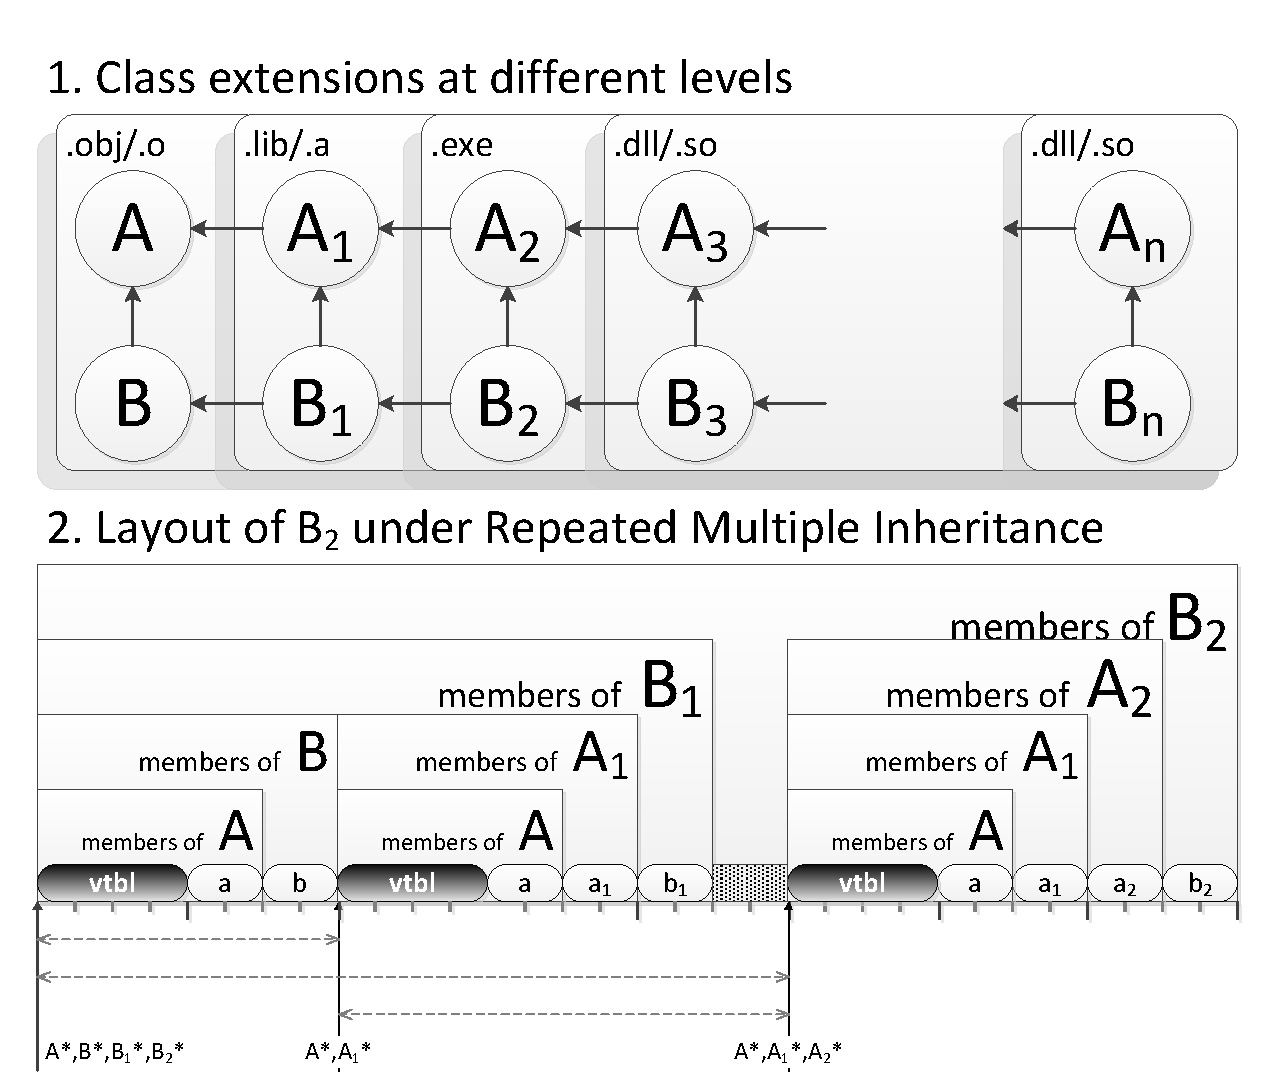
\includegraphics[width=0.47\textwidth]{Repeated.pdf}
  \caption{Casts under Open World Assumption}
  \label{fig:repeated}
\end{figure}

Historically, because of compatibility with C and its toolchain, the C++ 
compilers could never rely on advanced linkers. This is why they always had to 
generate code under \emph{open world assumptions} -- any class hierarchy is 
potentially unbound and no tool in the chain may assume seeing the entire 
hierarchy, including the loader. This made C++ compilers interoperable with 
other languages, truly modular and fast, but naturaly had its cons too.

To see why casting and type inclusion tests are not independent under the open 
world assumption, consider a translation unit declaring two classes \code{B <: A} 
and an object \code{a} of static type \code{A*}. Consider now an if-statement
\code{if (instanceof<B*>(a)) ...}, where hypothetical \code{instanceof} function only 
returns a boolean. Seeing that \code{B} is derived from \code{A} via single 
inheritance and thus knowing \code{A} is going to be at offset 0 of \code{B} it 
might be tempting to generate a code in the then-branch, that uses value of 
\code{a} as a \code{B*}. Unfortunately this is not correct. To understand why, 
consider a different module (e.g. static library) that extends both \code{A} and 
\code{B} with classes \code{A1} and \code{B1} as shown in 
Figure~\ref{fig:repeated}(1). The extension may not necessarily stop there: further 
extensions in similar manner may happen in the actual executable linking the 
original translation unit, static library and some other translation unit 
extending the library's extension further. An object created as 
\code{A* a = (A2*)new B2;} will satisfy the predicate \code{instanceof<B*>(a)} 
because \code{B} is unambiguous base class of \code{a}'s most-derived type, but 
clearly reinterpreting such pointer as \code{B} is incorrect, because \code{a} will 
be pointing to the third \code{A} of \code{B2} and pointer adjustment is needed.

This example illustrates that under open world assumption, the C++ compiler must 
in general always assume presence of repeated inheritance. It also explains why 
C++ uses a slow but open link chasing algorithm to implement its 
\code{dynamic_cast} operator and advocates for studying the complexity of 
combined operation of type testing and type casting. 

\subsection{The Source of Inefficiency}

Leaving aside non-opennes of some techniques for type inclusion testing we would 
like to show that their use to implement type switch is inferior to some 
workaround techniques, also not open, which may prevent a language 
implementation of such a switch not be adopted due to inferior performance.

We implemented several constant-time subtype testing techniques for a given 
class hierarchy and then compared it with several known workarounds.

\begin{figure}[htbp]
  \centering
    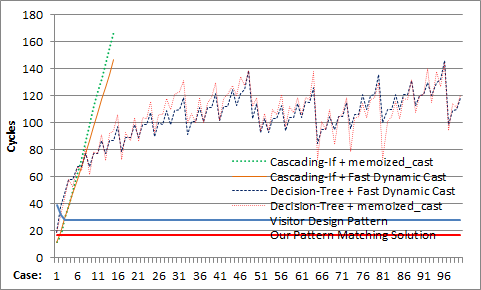
\includegraphics[width=0.47\textwidth]{DCast-vs-Visitors2.png}
  \caption{Type switching based on the fast dynamic cast of Gibbs and Stroustrup~\cite{FastDynCast}}
  \label{fig:DCastVis2}
\end{figure}

As can be seen from the picture in Figure~\ref{fig:DCastVis2}, the logarithmic 
cost associated with the decision tree very quickly surpasses the time visitor 
design pattern or switch on tags takes to implement case analysis.